\section{Data}
We seek to calibrate the bi-partite random walker model, and thus find the strongest signal on the collaborative structure of open collaboration. For that, we have to find values of $\alpha$ and $\beta$, which minimize the distance between rankings given by the model and some ground-truth metrics on editor expertise and article quality, obtained independently from the input matrix. We perform the model calibration for 13 snapshots (see Figure \ref{fig:snapshots})  for each of  the 12 categories of Wikipedia articles presented in Table \nolinebreak \ref{tab:statistics}. We have selected a spectrum of categories ranging from anarchy and edit-warring (e.g., {\it Sexual Acts}) to acknowledged high organization level (e.g., {\it Military history of the US})


For each category and snapshot, we build the binary matrix $M_{ea}$ by parsing all edit histories of all articles up to the snapshot time. We set $M_{ea} = 1$ for editor $e$ having modified article $a$, and $M_{ea} = 0$ otherwise. In order to eliminate page vandals, we considered only editors who made 5 or more edits to any article in the category. Even though they contribute greatly to the emergence of quality in Wikipedia \cite{}, we have not considered the discussion pages associated to each article. We also discarded all software robots (i.e. {\it bots}) that programmatically edit Wikipedia. 

\begin{table}
\begin{tabular}{|l|c|c|c|}
%\toprule
\hline
{\bf Category} &  {\bf Articles} &  {\bf Editors} &  {\bf Edits} \\
%\midrule
\hline
American male novelists               &      2,460 &   9,946 &  224,783 \\
2013 films                            &      1,896 &   5,215 &  150,956 \\
American women novelists              &      1,936 &   5,968 &  138,716 \\
Nobel Peace Prize laureates           &       104 &   4,165 &   91,522 \\
Sexual acts                           &        93 &   2,190 &   45,901 \\
Economic theories                     &       212 &   1,145 &   28,658 \\
Feminist writers                      &       233 &   1,357 &   25,738 \\
Yoga                                  &       123 &    730 &   25,315 \\
Military history of the US &       180 &    854 &   20,172 \\
Counterculture festivals              &        66 &    578 &   10,515 \\
Computability theory                  &        92 &    272 &    7,117 \\
Bicycle parts                         &        70 &    210 &    4,981 \\
\hline
\end{tabular}
\caption{Size statistics of investigated Wikipedia categories sorted by total edits.}
\label{tab:statistics}
\end{table}

\begin{figure}[!t]
\centering
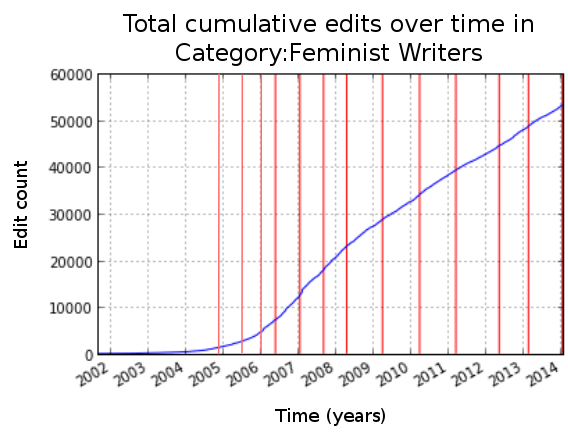
\includegraphics[width=0.9\columnwidth]{../Figures/cumulative_snapshots_Feminist_Writers_thirteen.png}
\caption{Cumulative edits made in Category {\it Feminist writers} (blue line). Vertical red lines represent the 13 snapshots taken at 2.5\%, 5\%, 7.5\% and then, 10\%, 20\%, 30\%, \ldots , 100\% of edits.}
\label{fig:snapshots}
\end{figure}

%\subsection{Editors Expertise and Articles Quality}
To calibrate $\alpha$ and $\beta$, we resorted to state-of-the-art ground-truth evaluations for editor expertise $\bar{w}_e$ and article quality $\bar{w}_a$. From these exogenous evaluations, we ranked editors and articles according to their expertise and quality respectively. We then performed  a grid search for values of $\alpha^*$ and $\beta^*$, which maximize the Spearman rank-correlation $\rho_e$ and $\rho_a$ between rankings obtained from the bi-partite random walker model $(w_e,w_a)$ and from exogenous metrics $(\bar{w}_e,\bar{w}_a)$. Actually, $(\alpha^*,\beta^*)$ must maximize both $\rho_e$ and $\rho_a$, even though $\rho_e$ and $\rho_a$ might actually be different. The optimization function  of $(\alpha^*,\beta^*)$ is given by,

\newcommand{\argmax}{\arg\!\max}

\begin{equation}
\begin{cases}
(\alpha^*,\beta^*) = \argmax_{\alpha, \beta}(\rho_e)\\
(\alpha^*,\beta^*) =\argmax_{\alpha, \beta}(\rho_a).\\
\end{cases}
\end{equation}

The set $(\alpha^*,\beta^*)$ characterizes how the structure of collaboration creates values in each Wikipedia category. To calibrate the model, we have used ground-truth metrics for article quality and editor expertise. 

A variety of techniques for measuring article quality have been proposed, from a collection of word-count related metrics \cite{blumenstock2008sizematters} to analyzing persistent and transient contributions throughout revisions\cite{woehner2009}. We have selected metrics used on Wikipedia \cite{wang2013tell,klein}, which have also been used in the CSCW literature in different combinations \cite{kane2011} \cite{keegan2012}. Our measure of actual article quality is performed through a combination of 5 text analysis metrics: (i) ratio of mark-up to readable text, (ii) number of headings, (iii) article length, (iv) citations per article length, (v) number of outgoing intra-Wiki links. We performed principal component analysis (PCA) for each category and snapshot in order to reduce dimensionality from 5 metrics to a single one (i.e. the principal component). The variance explained by the principal component varied between 0.5 and 0.72, confirming the dominance of the axis of maximum variance. Even though these five article quality metrics do not directly incorporate information from the bi-partite network (e.g. number of contributors, number of edits), they might indirectly be related, as some contributors specialize in some types of editing, such as adding citations or systematically improving the structure of articles \cite{}.

Editor expertise is even more difficult to address, as each article is a blend of the edits of several contributors, and disentangling remains a challenge, which has occupied Wikipedia researchers long before us, using techniques ranging from parsing the revision history to measuring text survival rate \cite{adler2008measuringauthor}. Although they are sophisticated, these metrics pose a variety of problems. For instance, some articles are likely to evolve not only because former editors introduced wrong statements, but simply because of new information brought to public attention. We decided to use ``labor hours" proposed by Geiger and Halfaker \cite{geiger2013}, which is calculated for each editor by taking contribution history up to the snapshot point. All edits made within $1$ hour of a previous edit are counted in an {\it edit session}. If more than one hour separates two edits, a new period of edits  starts. 
 The expertise expressed in labor hours is the sum of edit sessions. For the calculation of ground-truth expertise, we only consider edits for a given category, although the same editor might have edited other categories of articles in Wikipedia. The labor hours doesn't incorporate only the time effort spent by  editors on a Wikipedia category. It does not tell how this time is spent in the number (resp. size) of edits actually made during a period, or whether the effort has been spent on one or multiple articles. In other words, we cannot distinguish a single minded user spending $100$ hours on a single article trying to get it to ``Feature Article status" from a user making $100$ stub articles for $1$ hour each.  However, it is clear that a highly contributing editor has more chance to touch more articles over time, but the metric does not if some editors have rather edited the same articles. How this effort is distributed and brings quality is precisely what the {\it bi-partite random walker} model can say that other metrics cannot.  In a nutshell, parameters $\alpha$ and $\beta$ describe the most likely structure of collaboration given calibration of the model to ground-truth quality and expertise metrics. The higher the correlation between the model and the exogenous metrics, the better the collaboration structure is captured by the model. 

Finally, we shall discuss shortly the possibility that ground-truth article quality and editor expertise might be dependent. Again, it depends on the collaboration structure. In the extreme case where each article is produced by an editor, then the bi-partite random walker model collapses into a 1-dimensional problem, as well as the notion of collaboration. On the contrary, if all editors contribute to all articles, both editors and articles will all be equally ranked and the algorithm will not converge. A realistic solution lies in-between and is best captured by $\beta$.

% \textcolor{red}{Yet depending on our amount of preferential attachment in our network, one or the other could be seen as a superior editor. Likewise on pages, an article text can be changed in 5 ways. The same edits could be made by one generalist editor or 5 specialist editors, and the ground-truth would not change. Depending on a different preferential attachment parameter in the model could rank each of these very differently.}
%
%\textcolor{red}{Finally a point should be made about whether our exogenous expertise and quality measures are independent. Earlier on links between expert editors and quality articles were claimed \cite{wilkshuber}, and would seem intuitive. Yet, subsequently, there have been claims against such universal links which point out that key social interactions are not accounted for with these measures \cite{kane2009}. Intuitively this link rests on the collaborativeness of the articles and editors in question. With collaboration expertise will transtlate into article quality. However, given antagonistic, warring- editors expertise will not improve article quality.}

